\chapter{Experimental principles}\label{chap:2}

Before describing the specific techniques and hardware of the Fermilab Muon $g-2$ experiment, this chapter will outline the underlying physics principles of the measurement of anomalous magnetic momentum of the muon, $a_{\mu}$, and the search for the muon electric dipole moment. 

\section{Parity violation in weak interactions}\label{sec:ParityViolation} 

The ability to track the orientation of the muon's polarisation as a function of time is critical to both the measurement of $a_{\mu}$ and the muon EDM search. This orientation, however, is not directly observable: it can only be inferred from an understanding of parity violation in weak nuclear force. 

The notion that weak decays may not respect $P$-symmetry was first postulated by Lee and Yang in 1956 \cite{LeeAndYang}, and discovered soon after by Wu in 1957 \cite{Wu}. Lee and Yang were also the first to notice that this phenomenon could provide a means of studying the orientation of the muon's spin through the decay of pions into muons and muons to electrons\footnote{This section will hereafter exclusively refer to $\pi^{+}$, $\mu^{+}$, and $e^{+}$ (positrons), as these are most relevant to E989.}.

\begin{figure}[t!]
\centering{}
\includegraphics[trim={2.5cm 2cm 2cm 4.5cm},clip,width=\textwidth]{Images/Method/PionDecayCartoon.pdf}
\caption{A cartoon of a $\pi^{+}$ decay to a $\mu^{+}$ and a $\nu_{\mu}$, in the $\pi^{+}$ rest frame, illustrating the helicity configurations of the decay products. The effectively massless $\nu_{\mu}$ must have a left-handed (LH) configuration within the SM (with its spin and momentum antiparallel), and conservation of angular momentum requires that the $\mu^{+}$ is also produced with a LH configuration.}
\label{fig:PionDecay}
\end{figure} 

Positive pions, $\pi^{+}$, decay through the weak interaction into antimuons, $\mu^{+}$, and muon-neutrinos, $\nu_{\mu}$, by 
%
\begin{equation}
  \pi^{+}\rightarrow\mu^{+}+\nu_{\mu},
  \label{eqn:PionDecay}
\end{equation}
%
with a branching fraction of $>$99.9\% \cite{PDG2018}. The weak force exclusively couples to `left-handed' (LH) particles and `right-handed' (RH) antiparticles, where handedness refers to the particle's chirality. In the massless limit, chirality is equivalent to helicity: the component of a particle's spin along its direction of flight, $\hat{p}\cdot\hat{s}$.  A massless particle with LH helicity is one whose spin and momentum vectors lie anti-parallel, while the reverse is true for a RH massless particle. Neutrinos may be treated as effectively massless within the SM, so the $\nu_{\mu}$ produced in the $\pi^{+}$ decay has a LH helicity configuration. Pions are spin-0 particles, with no intrinsic angular momentum, so the $\mu^{+}$ spin vector must have the opposite orientation to the $\nu_{\mu}$ spin vector in order to conserve angular momentum. Since, in a two-body decay, the rest frame momentum vectors of the decay products oppose one another, the $\mu^{+}$ is produced with its spin and momentum antiparallel (with LH helicity). Such decays are sometimes called `backwards decays', illustrated in Figure \ref{fig:PionDecay}. A $\pi^{-}$ decay would produce a RH `forwards' going $\mu^{-}$.

\begin{figure}[t!]
\centering{}
\includegraphics[trim={2cm 2cm 2cm 4.5cm},clip,width=\textwidth]{Images/Method/MuonDecayCartoon.pdf}
\caption{A diagram of muon decay in the case where the energy of the decay positron is maximised. Conservation of angular momentum results in a preference for the spin vector of high energy decay positrons to be aligned with that of the parent muon.}
\label{fig:MuonDecay}
\end{figure}

Helicity is not Lorentz invariant, so, in the laboratory frame, muons are produced with a correlation between the orientation of their spin and momentum vectors, rather than with them perfectly antiparallel. Even so, this correlation makes it possible to produce a highly polarised muon beam by selecting those muons with the highest momentum (in the limit $v\rightarrow c$ the beam would be 100\% polarised). In this way, the initial orientation of the spin polarisation vector may be known. 

Following a rest frame lifetime of \SI{2.2}{\micro\second}, nearly 100\% of the $\mu^{+}$ will decay, again via the weak interaction, by
%
\begin{equation}
  \mu^{+} \rightarrow e^{+}+\nu_{e}+\bar{\nu}_{\mu},
  \label{eqn:MuonDecay}
\end{equation}
%
where the $\nu_{e}$ and $\bar{\nu}_{\mu}$ have LH and RH helicity configurations respectively \cite{PDG2018}. In the case where the $e^{+}$ energy is maximised, with a rest frame energy of $m_{\mu}/2$, the two neutrinos carry the remaining energy in the opposite direction to the $e^{+}$ (so their momentum vectors are aligned). In this configuration, illustrated in Figure \ref{fig:MuonDecay}, the two neutrinos have antiparallel spin vectors with a net angular momentum of zero. In order to conserve the $\mu^{+}$ angular momentum, the $e^{+}$ spin must be aligned with that of the parent $\mu^{+}$, giving it a RH helicity. The reverse is true in the situation where $e^{+}$ energy is minimised, where in this case the $e^{+}$ spin must be antiparallel with that of the parent $\mu^{+}$. Again, helicity is not Lorentz invariant, so the result in the laboratory frame is an energy dependent correlation between the direction the $e^{+}$ momentum and $\mu^{+}$ spin. This means that energy of the decay positrons encodes information about the orientation of the muon spin vector at the time of decay. %This is pivotal for any $g-2$ experiment, which, as will be explained, rely on measuring that exact quantity. %, where those with the highest energy the smallest emission angle between 

\section{Measuring $a_{\mu}$}

\subsection{Larmor precession}\label{sec:LarmorPrecession}

A muon placed in an external magnetic field, $\vec{B}$, will experience a torque which depends on its magnetic moment, $\vec{\tau}=\vec{\mu}\times\vec{B}$, inducing a rotation of the spin vector about the magnetic field lines. In the muon rest frame, the angular frequency of spin-precession, $\omega_{s}$, is given by the Larmor frequency:
%
\begin{equation} 
  \vec{\omega}_{s} = g_{\mu}\frac{Qe}{2m}\vec{B}.
  \label{eqn:Larmor}
\end{equation}
%
From this expression, it can be deduced that $g_{\mu}$ may be measured by injecting non-relativistic muons into a magnetic field and performing a simultaneous measurements of $\omega_{s}$ and $B$, where $\omega_{s}$ is determined by making use of the correlation between decay $e^{\pm}$ energy and spin orientation from the parity violation arguments outlined in the previous section. 

\subsection{The anomalous precession frequency, $\omega_{a}$}

A muon moving through a homogeneous magnetic field will not only undergo Larmor precession, at an angular frequency $\omega_{s}$, but will also be subject to the Lorentz force; causing it to travel in a circle of constant radius. This is cyclotron motion, where the angular cyclotron frequency, $\omega_{c}$, is defined by 
%
\begin{equation}
  \vec{\omega}_{c}=\frac{Qe}{m_{\mu}}\vec{B}.
  \label{eqn:Cyclotron}
\end{equation}
%
Remarkably, the difference between $\omega_{c}$ and $\omega_{s}$ has a direct dependence on the muon magnetic anomaly, $a_{\mu}=(g_{\mu}-2)/2$. This relative frequency is the anomaly frequency, $\omega_{a}$, defined as follows:
%
\begin{equation}
  \vec{\omega}_{a}=\vec{\omega}_{s}-\vec{\omega}_{c}=\left( \frac{g_{\mu}}{2}-1 \right)\frac{Qe}{m}\vec{B}=a_{\mu}\frac{Qe}{m}\vec{B}.
  \label{eqn:omega_a}
\end{equation}
%
A illustration of a population of spin polarised muons undergoing both Larmor precession and cyclotron motion in a constant magnetic field, in the case where $g_{\mu}=2$ ($\omega_{a}=0$) and $g_{\mu}\neq2$ ($\omega_{a}\neq0$), is shown in Figure \ref{fig:AnomalyFreq}. 

\begin{figure}[t!]
\centering{}
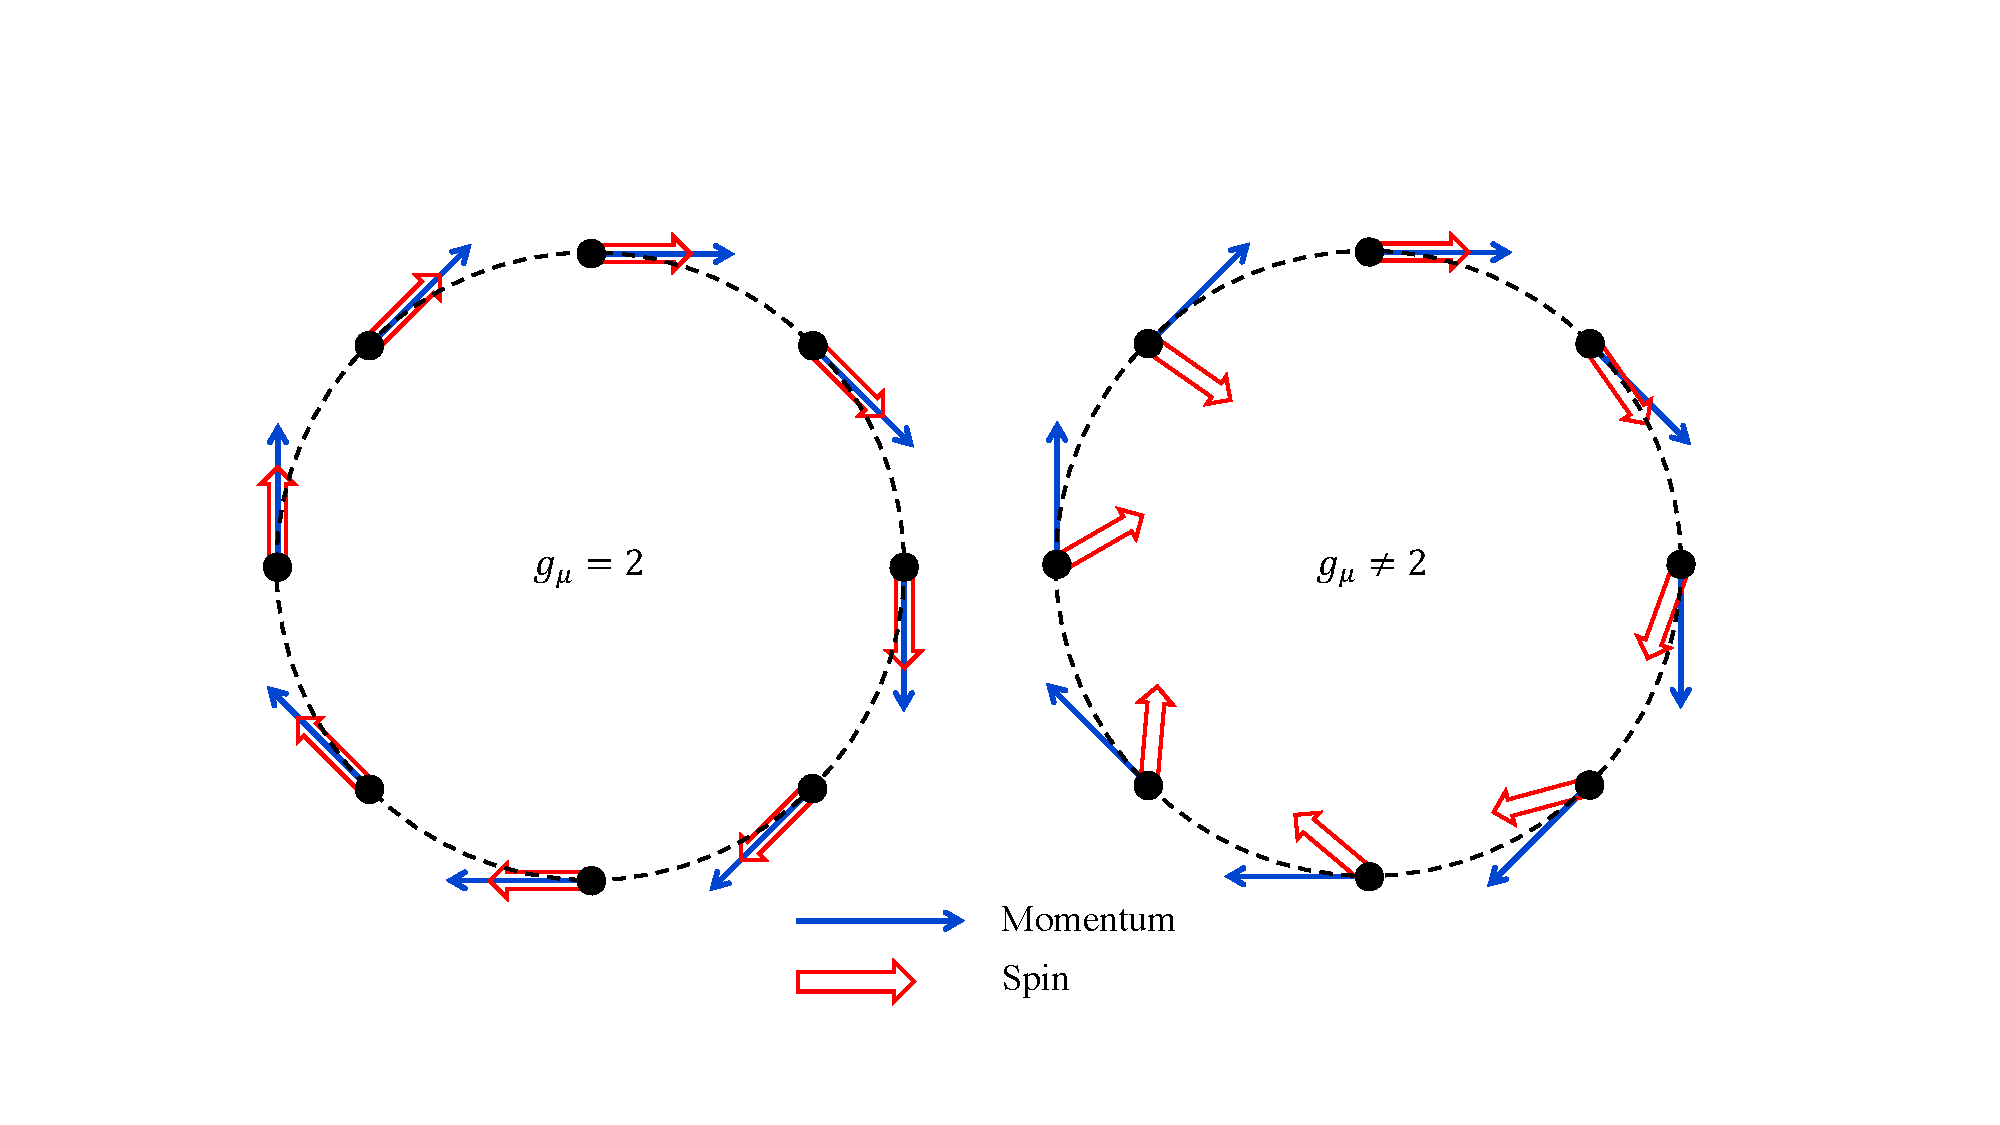
\includegraphics[trim={2cm 2cm 2cm 2cm},clip,width=\textwidth]{Images/Chapter2/AnomalyFrequencyCartoon.pdf}
\caption{An illustration of the relative precession of the spin polarisation and momentum vectors of a muon traversing a constant magnetic field, where the magnetic field lines are directed out of the page and the muons are injected at 12 o'clock. If $g_{\mu}=2$, then the two vectors will remain in phase; if $g_{\mu}\neq2$ then they will move out of phase. The rate of precession of the spin vector relative to the momentum vector is the anomaly frequency, $\vec{\omega}_{a}$, enabling a direct measurement of $a_{\mu}$.} 
\label{fig:AnomalyFreq}
\end{figure}

\subsection{Measuring $\omega_{a}$}

The anomaly frequency is measured by making use of the parity violation arguments outlined in Section \ref{sec:ParityViolation}, which give a correlation between $e^{+}$ emission angle and $\mu^{+}$ spin vector which depends on the $e^{+}$ energy. Because of this, the population of high energy $e^{+}$ will vary as a function of time with a frequency equal to $\omega_{a}$, where the maxima of the oscillation will occur when the muon spin and momentum vectors are aligned, and the minima when they are antialigned. The choice of low energy threshold used to define `high energy $e^{+}$' is discussed in Section \ref{subsec:SensitivityToOmegaA}. The anomalous precession oscillation may be fitted with a sinusoidal function in order to extract the frequency, which is illustrated by use of a toy model in Figure \ref{fig:ToyWiggle}. 

\begin{figure}[t!]
\centering{}
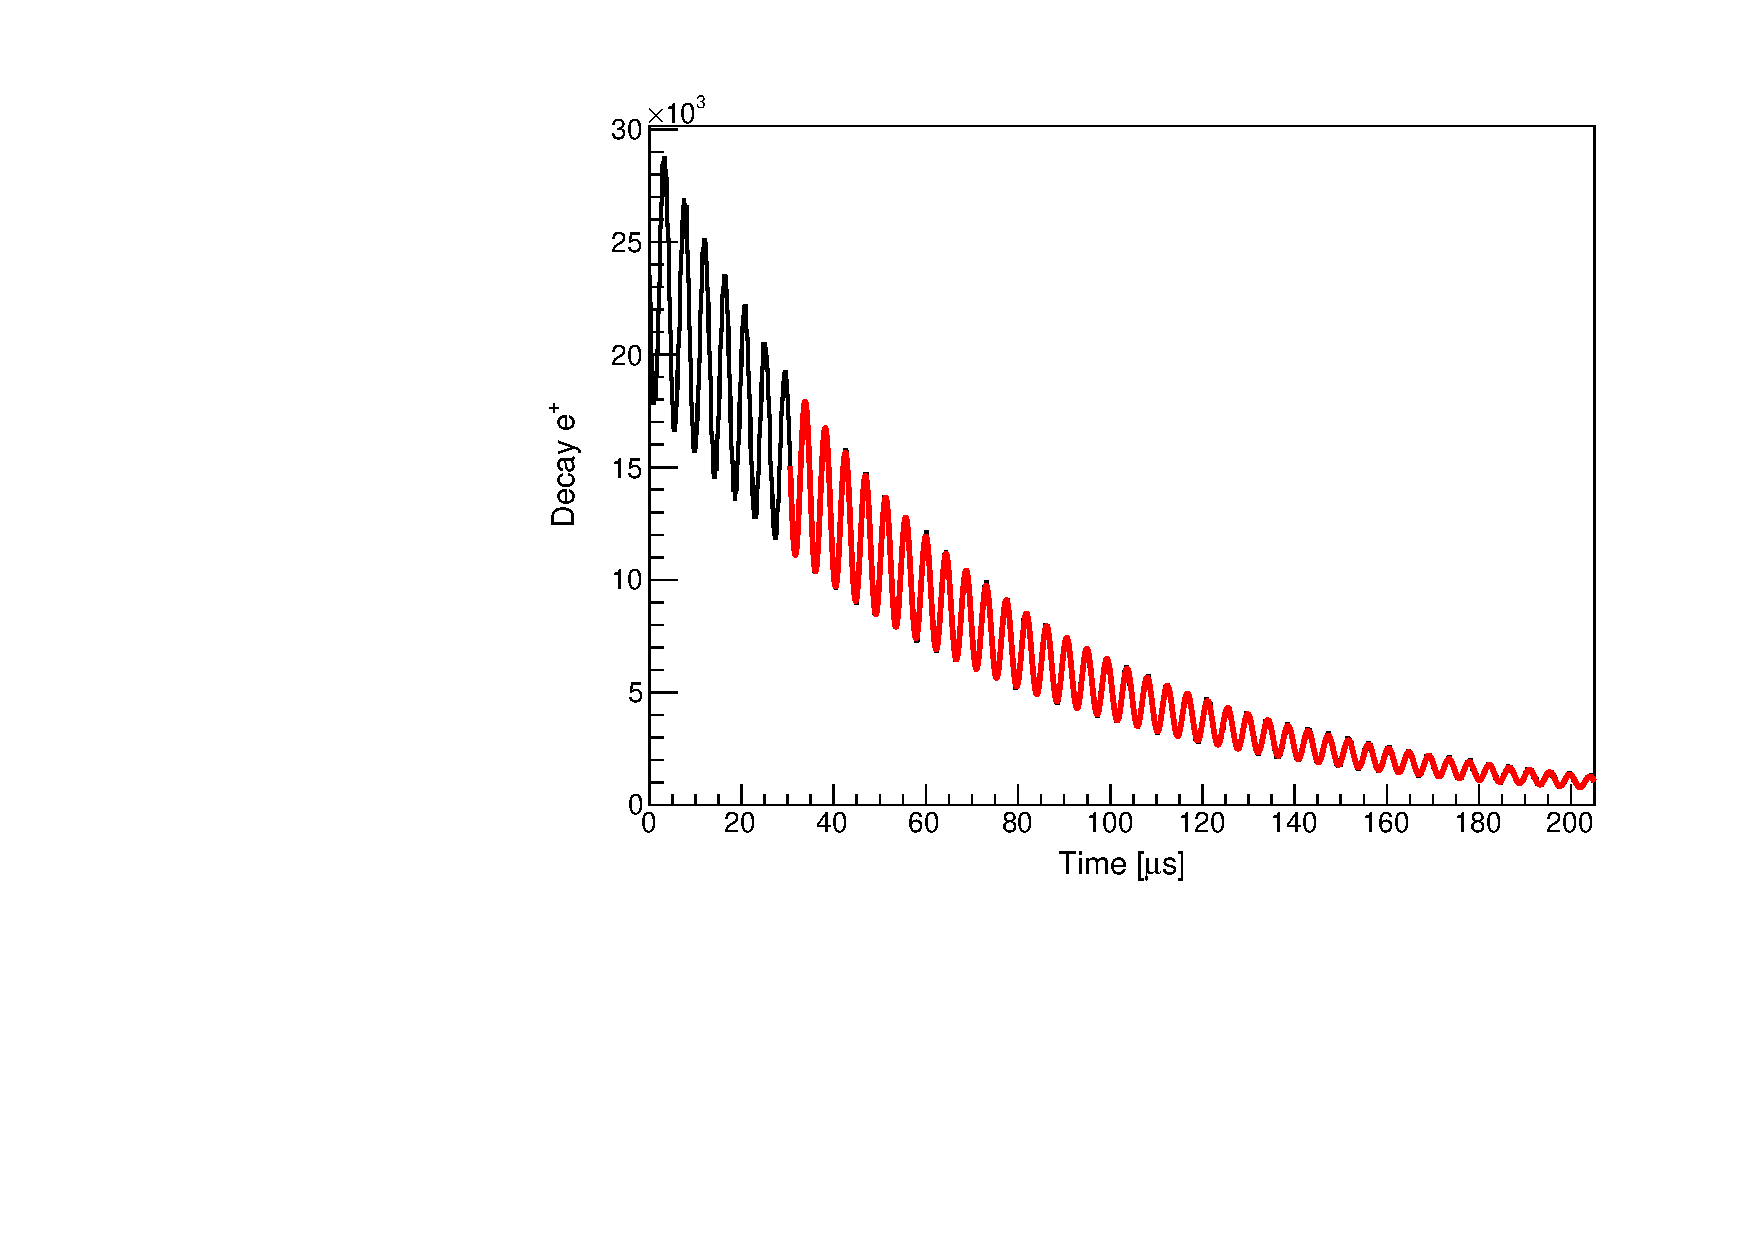
\includegraphics[trim={0cm 0cm 0cm 0cm},clip,width=.69\textwidth]{Images/Chapter2/ToyWiggle.pdf}
\caption{A toy model of the subset of high energy $e^{+}$ emitted from an exponentially decaying population of muons, varying at the anomaly frequency, $\omega_{a}$, which is extracted from the data by use of a sinusoidal fit (illustrated by a red curve).}
\label{fig:ToyWiggle}
\end{figure}

\subsection{Corrections to $\omega_{a}$}\label{sec:OmegaACorrections}

It is highly advantageous to use relativistic muons when conducting a measurement of $a_{\mu}$, or the muon EDM, not least because this allows for a longer measurement period due to the dilation of laboratory frame muon lifetime by factor of $\gamma$ (the Lorentz factor, $1/\sqrt{1-v^{2}/c^{2}}$). For relativistic muons, the Larmor precession angular frequency must be corrected to account for the relative rotation of the muon rest frame and the laboratory frame. This correction is known as Thomas precession \cite{ThomasPrecession}, where the modified angular spin-precession frequency is given by
%
\begin{equation}
  \vec{\omega}_{s} = g_{\mu}\frac{Qe}{2m_{\mu}}+(1-\gamma)\frac{Qe}{m_{\mu}\gamma}\vec{B}.
  \label{eqn:ThomasPrecession}
\end{equation}
%
The cyclotron angular frequency also receives a relativistic correction, by
%
\begin{equation}
  \vec{\omega}_{c} = g_{\mu}\frac{Qe}{\gamma m_{\mu}}\vec{B},
  \label{eqn:RelativisticCycltron}
\end{equation}
%
resulting in a modified expression for $\omega_{a}$:
%
\begin{equation}
  \vec{\omega}_{a} = g_{\mu}\frac{Qe}{2m_{\mu}}+(1-\gamma)\frac{Qe}{m_{\mu}\gamma}\vec{B} - g_{\mu}\frac{Qe}{\gamma m_{\mu}}\vec{B}.
  \label{eqn:RelativisticOmegaA}
\end{equation}
%
The relativistic parts of the above equation cancel, returning a simplified expression equal to the non-relativistic Equation \ref{eqn:omega_a}. 

As a further complication, the E989 storage ring employs electrostatic quadrupoles (ESQs) to provide vertical focusing to the beam -- discussed in detail in Chapter \ref{chap:3} Section \ref{sec:ESQs}. The presence of an external electric field, $\vec{E}$, modifies both $\omega_{s}$ and $\omega_{c}$ again, so that $\omega_{a}$ is described by
%
\begin{equation}
  \vec{\omega}_{a}=\frac{Qe}{m_{\mu}} \left[ a_{\mu}\vec{B}-a_{\mu}\left(\frac{\gamma}{\gamma+1}\right)(\vec{\beta}\cdot\vec{B})\;\vec{\beta}-\left(a_{\mu}-\frac{\gamma}{1-\gamma^{2}}\right) (\vec{\beta} \times \vec{E}) \right]. %(\vec{\beta}\times\vec{E}) 
  \label{eqn:FullOmega_a}
\end{equation}
%
Two steps can be taken to simplify Equation \ref{eqn:FullOmega_a}. The first is use the approximation $\beta\cdot\vec{B}\approx0$, where the muon momentum vector is assumed to be orthogonal to the magnetic field lines, reducing the second term to zero. This assumption holds when averaging over the full orbit, but vertical betatron oscillations\footnote{Discussed further in Chapter \ref{chap:3} Section \ref{sec:BeamDynamics}.} introduce periodic changes in the `pitch' of the muon momentum vector: necessitating a small correction to $\omega_{a}$, known as the pitch correction. The second step is to select a value of $\gamma$ such that
%
\begin{equation}
  \gamma=\sqrt{1+\frac{1}{a_{\mu}}},
  \label{eqn:MagicGamma}
\end{equation}
%
which is often referred to as the `magic' $\gamma$, corresponding to a momentum of 3.094 GeV\footnote{Momentum will be expressed in natural units, where $\hbar=c=1$, throughout this thesis.}, or the `magic' momentum, which reduces the third term to zero. In practice, the muon momentum is distributed about the magic momentum with a width of $\pm$0.15\%, so that an additional correction, termed the E-field correction, is required to accurately measure $\omega_{a}$. Further reading on these corrections, as applied to E989 Run-1 data, can be found in \cite{OmegaARun1} and \cite{BeamDynamics}.

\subsection{Sensitivity to $\omega_{a}$}\label{subsec:SensitivityToOmegaA}
% 
As discussed previously, the $\omega_{a}$ signal arises from the energy dependent correlation between the orientation of the parent muon spin vector and the decay positron momentum vector. This relationship will be referred to here as the decay asymmetry, and it must be optimised with carefully selected energy cuts in order to maximise sensitivity to $\omega_{a}$. If positrons across the full energy spectrum were counted, then all that would be observed would be a pure exponential from the decaying muon population; whereas if only positrons with maximum energy were counted, the decay asymmetry would be maximised, but the number of positrons collected would be extremely small and the statistical uncertainty very high. The correct approach is to choose a low energy threshold which gives the optimum balance between decay asymmetry and statistical sensitivity. 

\begin{figure}[b!]
\centering{}
\subfloat[Rest frame.]{\includegraphics[trim={0 0 0 0},clip,width=0.49\textwidth]{Images/Method/Asymmetry_wa_restFrame.pdf}\label{subfig:Asymmetry_wa_restFrame}} \hfill
\subfloat[Laboratory frame.]{\includegraphics[trim={0 0 0 0},clip,width=0.49\textwidth]{Images/Method/Asymmetry_wa_labFrame.pdf}\label{subfig:Asymmetry_wa_labFrame} }
\caption{The number distribution function, $N$, the decay asymmetry function, $A$, and the statistical figure-of-merit function, $NA^{2}$, against fractional positron energy in (a) the muon rest frame and (b) the laboratory frame.}
\end{figure}    
%
%
\begin{figure}[t!]
\centering{}
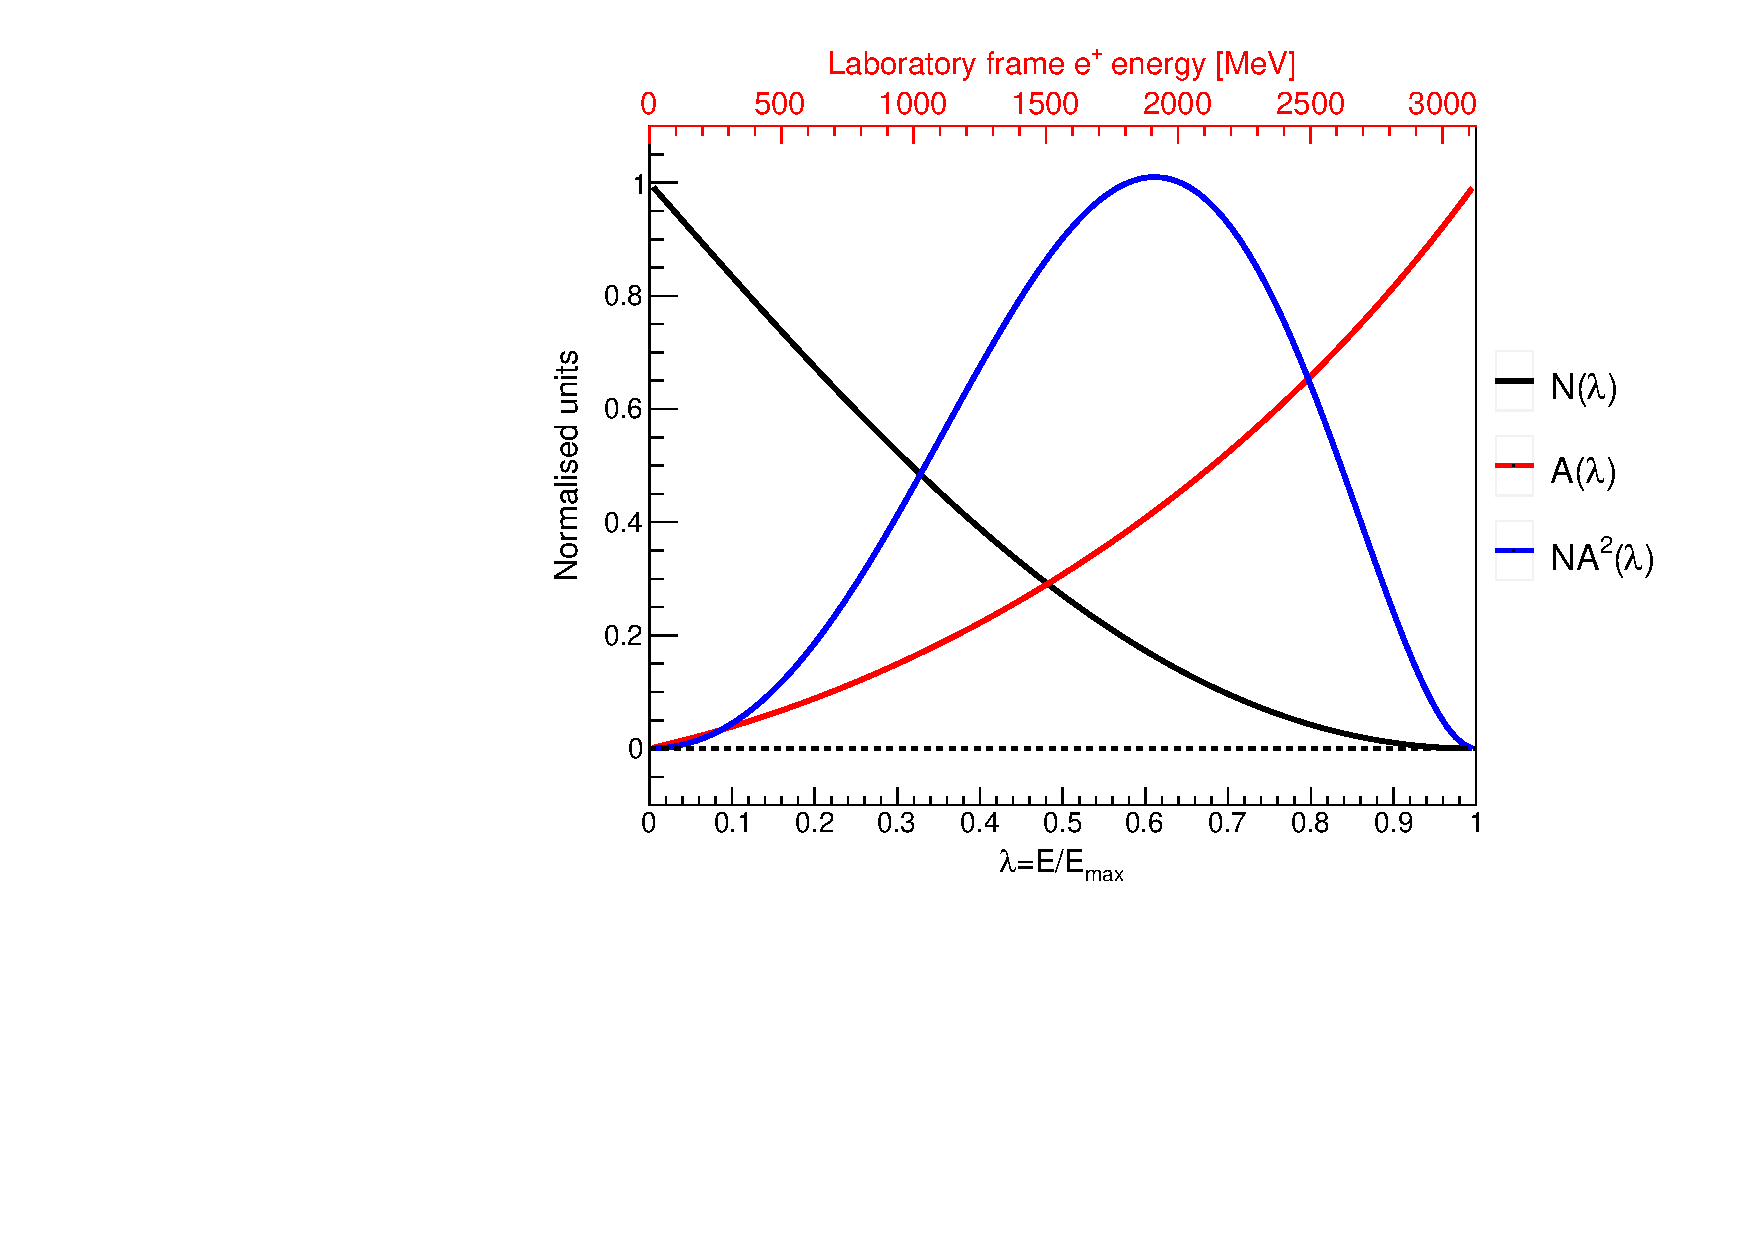
\includegraphics[trim={0 0 0 0},clip,width=.69\textwidth]{Images/Chapter2/Asymmetry_wa_labFrame_eCut.pdf}
\caption{The number distribution function, $N(\lambda)$, the decay asymmetry function, $A(\lambda)$, and the statistical figure-of-merit function, $NA^{2}(\lambda)$, in the laboratory frame; for a subset of positrons above some energy threshold.}
\label{fig:Asymmetry_wa}
\end{figure}  
%
In the muon rest frame, hereafter indicated by asterisks, the differential probability of positron emission into a solid angle $d\Omega^{*}$ is given by 
%
\begin{equation}
  dP(\lambda^{*}, \theta^{*}) \propto N(\lambda^{*})[1-A(\lambda^{*})\cos(\theta^{*})]d\lambda^{*} d\Omega^{*},
  \label{eqn:DiffDecay}
\end{equation}
%
where $\lambda^{*}=E^{*}/E_{max}^{*}$ (the positron fractional energy), $N(\lambda^{*})$ is the number distribution function (the number of positrons as a function of $\lambda^{*}$), $A(\lambda^{*})$ is the decay asymmetry function, and $\theta^{*}$ is the angle between the muon spin and positron momentum at the time of decay. Assuming that $E^{*}>>m_{e}$, $N(\lambda^{*})$ and $A(\lambda^{*})$ are given by
%
\begin{equation}
  N(\lambda^{*}) = 2\lambda^{*2}(3-2\lambda^{*}),
  \label{eqn:N_restFrame}
\end{equation}
%
and
%
\begin{equation}
  A(\lambda^{*}) = \frac{2\lambda^{*}-1}{3-2\lambda^{*}},
  \label{eqn:A_restFrame}
\end{equation}
%
which are illustrated in Figure \ref{subfig:Asymmetry_wa_restFrame}. Transforming into the laboratory frame and taking $\theta=\omega_{a}t+\phi$, where $\omega_{a}$ is the aforementioned anomalous spin precession angular frequency, $t$ is the time since injection discussed in Chapter \ref{chap:3} Section \ref{sec:InjectionAndStorage}, and $\phi(\lambda)$ is the phase as a function of laboratory frame fractional energy, gives the number oscillation as a function of time and energy,
%
\begin{equation}
  N(\lambda, t) = N_{0}(\lambda)e^{-t/\gamma\tau_{\mu}}[1+A(\lambda)\cos(\omega_{a}t+\phi(\lambda))].
  \label{eqn:FiveParFunc}
\end{equation}
%
The parameter $N_{0}$ in the above expression is the overall normalisation, $\tau$ is the muon lifetime in the rest frame, $\gamma$ is the `magic' Lorentz factor defined by Equation \ref{eqn:MagicGamma}, and $A(\lambda)$ is the laboratory frame decay asymmetry. This, Equation \ref{eqn:FiveParFunc}, is the basic five-parameter function used to extract $\omega_{a}$ via an unconstrained fit to the number oscillation above some energy threshold, the same expression used in the toy fit shown in Figure \ref{fig:ToyWiggle}. The laboratory frame number distribution function is given by 
%
\begin{equation}
  N(\lambda) = \frac{1}{3}(\lambda-1)(4\lambda^{2}-5\lambda-5),
  \label{eqn:N_labFrame}
\end{equation}
%
and the decay asymmetry function by
%
\begin{equation}
  A(\lambda) = \frac{1+\lambda-8\lambda^{2}}{4\lambda^{2}-5\lambda-5},
  \label{eqn:A_labFrame}
\end{equation}
%
both of which are illustrated in Figure \ref{subfig:Asymmetry_wa_labFrame}. For a subset of positrons above some energy threshold, $E_{th}$, these expressions must be modified again by integration from $\lambda_{th}$ to one, so that
%
\begin{equation}
  N(\lambda_{th}) = \frac{1}{3}(\lambda_{th}-1)^{2}(-\lambda_{th}^{2}+\lambda_{th}+3)
  \label{eqn:Nth_labFrame}
\end{equation}
%
and
%
\begin{equation}
  A(\lambda_{th}) = \frac{\lambda_{th}(2\lambda_{th}+1)}{3+\lambda_{th}-\lambda_{th}^{2}},
  \label{eqn:Ath_labFrame}
\end{equation}
%
which is shown in Figure \ref{fig:Asymmetry_wa}. 

The statistical uncertainty associated with $\omega_{a}$ may then be found by fitting the above-threshold number oscillation with the five-parameter function (Equation \ref{eqn:FiveParFunc}), which is inversely proportional to the statistical figure-of-merit (FOM) $NA^{2}$, by 
%
\begin{equation}
  \frac{\delta\omega_{a}}{\omega_{a}} = \frac{\sqrt{2}}{\omega_{a}\tau\sqrt{N}A},
  \label{eqn:OmegaAStatUnc}
\end{equation}
%
where $N$ refers to the total number of positrons. The ideal energy threshold is then the point where $NA^{2}$ is maximised \cite{BNLStatMethods}. Further discussion on this topic can be found in \cite{Miller_2007}. In E989, accounting for detector effects such as resolution and acceptance, this threshold is found to be 1.7 GeV \cite{OmegaARun1}.

\subsection{The final determination of $a_{\mu}$}

To make a determination of $a_{\mu}$, the magnetic field must also be measured to a high precision. In E989, this is accomplished by the use of nuclear magnetic resonance (NMR) magnetometers, called probes, where a simplified version of the procedure involves measuring the Larmor precession frequency of a free proton, $\omega_{p}$, which is used to relate the magnetic field by 
%
\begin{equation}
  \omega_{p} = 2\mu_{p} B, 
  \label{eqn:FreeProton}
\end{equation}
%
where $\mu_{p}$ is the magnetic moment of the proton. A detailed discussed of the E989 magnetic field system is given in Chapter \ref{chap:2} Section \ref{sec:Field}, as well as \cite{Field}. Combining Equation \ref{eqn:omega_a} and Equation \ref{eqn:FreeProton} allows for $a_{\mu}$ to be expressed in terms of $\omega_{a}$ and $\omega_{p}$, such that
%
\begin{equation}
  a_{\mu} = \frac{\omega_{a}}{\omega_{p}} \frac{2\mu_{p}m_{\mu}}{Qe}, 
\end{equation}
%
which can be rewritten in terms of the scalar electron magnetic moment
%
\begin{equation}
  \mu_{e} = g_{e}\frac{Qe}{4m_{e}}, 
\end{equation}
%
allowing $a_{\mu}$ to be written in terms of the two frequencies measured in the experiment and three well-measured ratios: 
%
\begin{equation}
  a_{\mu}=\frac{g_{e}}{2}\frac{\omega_{a}}{\omega_{p}}\frac{m_{\mu}}{m_{e}}\frac{\mu_{p}}{\mu_{e}}.
  \label{eqn:a_mu}
\end{equation}
%
As of 2018, $g_{e}$, $m_{\mu}/m_{e}$, and $\mu_{p}/\mu_{e}$ are known to within 0.00017 ppb, 22 ppb, and 0.3 ppb respectively \cite{CODATA_2018}. These uncertainties, with a quadrature sum of 22 ppb (compared with E989's target precision of 140 ppb), do not present any limitation to the precision on the final determination of $a_{\mu}$ at Fermilab. 

\section{Searching for a muon EDM}

\subsection{The spin precession plane tilt angle}

A muon with an electric dipole moment (EDM) of zero undergoing spin precession in a magnetic field will do so in the manner described previously: with its spin polarisation vector orthogonal to the magnetic field lines, as illustrated in Figure \ref{subfig:NoTilt}. However, if the muon EDM is non-zero, and the muon is relativistic, it will experience a torque due to the electric field induced by the Lorentz transformation of the laboratory magnetic field into the muon rest frame. In E989, external electric fields generated by the beam focusing electrostatic quadrupoles (ESQs), described in Chapter \ref{chap:3} Section \ref{sec:ESQs}, also contribute to this torque, resulting in a tilted precession plane where the angle between the polarisation vector and the magnetic field lines is directly related to the size of the muon EDM, $d_{\mu}$. An illustration of a tilted spin precession due to non-zero muon EDM is shown in Figure \ref{subfig:EDMTilt}.

A tilt in the spin precession plane resulting from a non-zero muon EDM would introduce an additional angular frequency, $\vec{\omega}_{\eta}$, orthogonal to $\vec{\omega}_{a}$, which is described in the approximation $\vec{\beta}\cdot\vec{E}\approx0$ (so that the muon momentum vector is orthogonal to the ESQ electric field, $\vec{E}$) by 
%
\begin{equation} 
  \vec{\omega}_{\eta} = \eta\frac{Qe}{2m}\left(\vec{\beta}\times\vec{B}+\frac{\vec{E}}{c}\right),
  \label{eqn:omega_eta}
\end{equation}
%
where $\eta$ is the dimensionless coupling between EDM and the spin described in Equation \ref{eqn:eta}, and the $\vec{\beta}\times\vec{B}$ term is representative of the influence of the induced electric field from the Lorentz transformation of the magnetic field. 
% %
\begin{figure}[t!]
\centering{}
\subfloat[No EDM.]{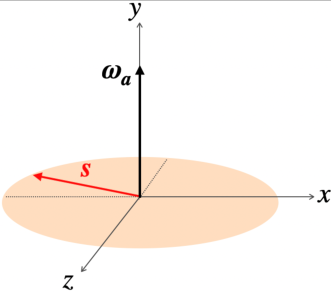
\includegraphics[trim={0 0 0 0},clip,width=0.47\textwidth]{Images/Chapter2/NoTilt.pdf}\label{subfig:NoTilt} } \hfill
\subfloat[Non-zero EDM.]{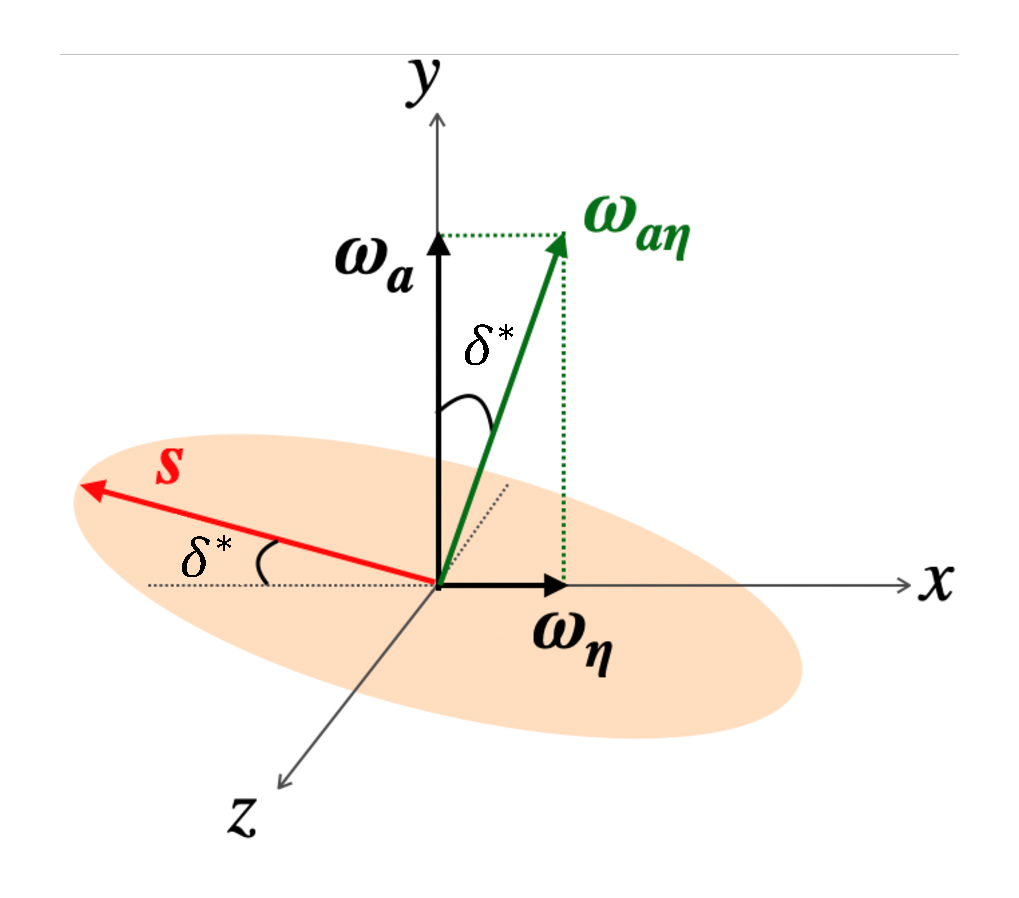
\includegraphics[trim={0 0 0 0},clip,width=0.47\textwidth]{Images/Chapter2/EDMTilt2.pdf}\label{subfig:EDMTilt} }
\caption{The muon spin precession plane with in the case of (a) no EDM and (b) a non-zero EDM, where the plane is tilted in the muon rest frame by a maximum angle $\delta^{*}$. The magnetic field lines are directed along the y-axis and the z-axis is aligned with the direction of motion in the laboratory frame. Images courtesy of R. Chislett \cite{BeckyGeometry}.}
\label{fig:Tilt1}
\end{figure}
% %
In rest frame of the muon (again, indicated by asterisks), the spin precession plane tilt angle, $\delta^{*}$, is given by
%
\begin{equation} 
  \delta^{*} = \tan^{-1}\left(\frac{\omega_{\eta}}{\omega_{a}}\right) = \tan^{-1}\left(\frac{\eta\beta}{2a_{\mu}}\right), \label{eqn:delta_rest}
\end{equation}
%
which may be transformed into the laboratory frame by letting $\vec{\omega}_{\eta}$ be directed along the $x$-axis and $\vec{\omega}_{\eta}$ along the $y$-axis, so that $\delta^{*}$ may be written as 
%
\begin{equation} 
  \delta^{*} = \tan^{-1}\left(\frac{\Delta{x}^{*}}{\Delta{y}^{*}}\right),
  % \label{eqn:delta_rest}
\end{equation}
%
where $\Delta{x}^{*}$ and $\Delta{y}^{*}$ may be Lorentz boosted to the laboratory frame by
%
\begin{equation} 
  \Delta{x} = \frac{\Delta{x}^{*}}{\gamma} \quad \text{and} \quad \Delta{y} = \Delta{y}^{*}.
  % \label{eqn:delta_rest}
\end{equation}
%
The expression for the laboratory frame tilt angle, $\delta$, is then 
%
\begin{equation} 
  \delta = \tan^{-1}\left(\frac{\Delta{x}^{*}}{\gamma\Delta{y}^{*}}\right) = \tan^{-1}\left(\frac{\tan{\delta^{*}}}{\gamma}\right),
  \label{eqn:delta_lab}
\end{equation}
%
which is reduced compared the rest frame. In practice, the small angle approximation may be applied, so that this reduction is simply equal to a factor of $1/\gamma$. Finally, the relationship between the $d_{\mu}$ and $\delta$ may be found by combining Equations \ref{eqn:eta}, \ref{eqn:delta_rest}, and \ref{eqn:delta_lab}, so that
%
\begin{equation} 
  d_{\mu} = \frac{Qe\gamma\hbar a_{\mu}}{2m_{\mu}c\beta}\tan{\delta}.
  \label{eqn:EDMFromAngle}
\end{equation}
%
\subsection{The change in $a_{\mu}$ due to a muon EDM}\label{subsec:amuEDM}

The oscillation induced by a non-zero EDM increases the total angular frequency of spin precession, $\omega_{a\eta}$, by
%
\begin{equation} 
  \omega_{a\eta} = \sqrt{\omega_{a}^{2}+\omega_{\eta}^{2}} 
\label{eqn:omega_aeta}
\end{equation}
%
In principle, this means that non-zero muon EDM could account for the observed deviation in $a_{\mu}$, where the value of $d_{\mu}$ required may be estimated by equating the necessary fractional increase in spin precession frequency to the fractional deviation in $a_{\mu}$. The resulting EDM for a discrepancy $\Delta a_{\mu}$ may then be estimated by the expression
%
\begin{equation}
    d_{\mu} = \sqrt{\Delta a_{\mu}}\cdot \frac{a_{\mu}^{\text{Exp}}}{\sqrt{a_{\mu}^{\text{SM}}}} \cdot\frac{\hbar e }{\sqrt{2}m_{\mu} c \beta },
    \label{eqn:dmu_shift}
\end{equation}
%
for which a full derivation is given in Appendix \ref{app:amuEDMDerivation}. 

Taking the values of $a_{\mu}^{\text{Exp}}$, $a_{\mu}^{\text{SM}}$, and $\Delta a_{\mu}$ stated in Chapter \ref{chap:1} Section \ref{sec:TheMDM}, and attributing the entirety of $\Delta a_{\mu}$ to $d_{\mu}$, gives a muon EDM with a value 
%
\begin{align*}
d_{\mu} = (2.3\pm0.3)\times10^{-19}\,e\cdot\text{cm}.
\end{align*} 
%
This exceeds the current upper limit of $|d_{\mu}| < 1.8\times10^{-19}\,e\cdot\text{cm}\text{ (95\% C.L.)}$ \cite{BNLEDM}, meaning that the probability of $\Delta a_{\mu}$ being driven entirely by a non-zero muon EDM is less than 5\%. Moreover, this is $\mathcal{O}(10^{10})$ larger than the current upper limit on the electron EDM\footnote{Or, $\mathcal{O}(10^{8})$ larger than the corresponding indirect upper limit on the muon EDM, assuming the linear mass scaling discussed in Chapter \ref{chap:1} Section \ref{sec:TheEDM}.} \cite{ImprovedElectronEDMLimit}, and is beyond the realms of BSM models which allow for a large muon EDM. Any remaining ambiguity as to a contribution to $\Delta a_{\mu}$ from $d_{\mu}$ further motivates the muon EDM search at E989.

\subsection{The vertical decay angle based search}\label{subsec:VerticalAngleBasedSearch}

A number of approaches exist for measuring $\delta$, but this work will focus on a search technique based on a direct measurement of the oscillation in the average vertical angle of decay positrons by use of two straw tracker detectors. The equivalent tracker-based analysis at BNL, called the `traceback analysis', was statistically limited, rather than systematically limited as the calorimeter-based methods were \cite{BNLEDM}: meaning that a tracker-based EDM search at Fermilab offers obvious potential for an improvement in sensitivity over BNL, due the availability of a much larger integrated dataset\footnote{Note that this does not necessarily mean that the calorimeter-based methods are inferior to the tracker-based method.}. The E989 detector systems, including the straw trackers, are introduced in Chapter \ref{chap:3} Section \ref{sec:Detectors}, and an overview of the E989 datasets is provided in Chapter \ref{chap:3} Section \ref{sec:MeasPeriods}.

As with the measurement of $\omega_{a}$, this method relies on the energy dependent correlation between the muon spin vector and the momentum vector of the decay positron. In the context of a muon undergoing spin precession with tilted precession plane, this correlation would result in an oscillation in the average vertical decay angle of emitted positrons at an angular frequency $\omega_{a\eta}$. The vertical decay angle, $\theta_{y}$, is defined in this thesis as the angle that momentum vector makes with the $x$-$z$ plane in the laboratory frame, so that 
%
\begin{equation}
  \theta_{y} = \sin^{-1}\left(\frac{p_{y}}{p}\right).
  \label{eqn:theta_y}
\end{equation}
%As noted previously, the maxima and minima of the $\omega_{a}$ oscillation occurs when the muon spin and momentum either are aligned or antialigned. In the case of the $\omega_{\eta}$ oscillation the maxima and minima occur when the tilt angle is maximised: when the spin vector is orthogonal to the momentum vector. As a result of this, the oscillation in $\langle \theta_{y} \rangle$ is $\pi/2$ out-of-phase with $\omega_{a}$ -- a useful property, given that the anomalous precession oscillation phase is an easily measurable quantity. 

As noted previously, the maxima and minima of the $\omega_{a}$ oscillation occurs when the muon spin and momentum either are aligned or antialigned. In the case of the $\omega_{\eta}$ oscillation the maxima and minima occur when the tilt angle is maximised: when the spin vector is orthogonal to the momentum vector. As a result of this, the oscillation in average vertical angle, $\langle \theta_{y} \rangle$, is $\pi/2$ out-of-phase with $\omega_{a}$. To then begin extracting $\delta$, the average vertical angle, $\langle\theta_{y}\rangle$, must be fitted with a function consisting of two orthogonal terms, plus a constant offset, $c$, as follows:
%
\begin{equation}
  \langle\theta_{y}\rangle(t)=A_{g-2}\cos(\omega_{a}t+\phi)+A_{\text{EDM}}\sin(\omega_{a}t+\phi) + c,   
  \label{eqn:VertAngleFitFunc}
\end{equation}
%
\begin{figure}[t!]
\centering{}
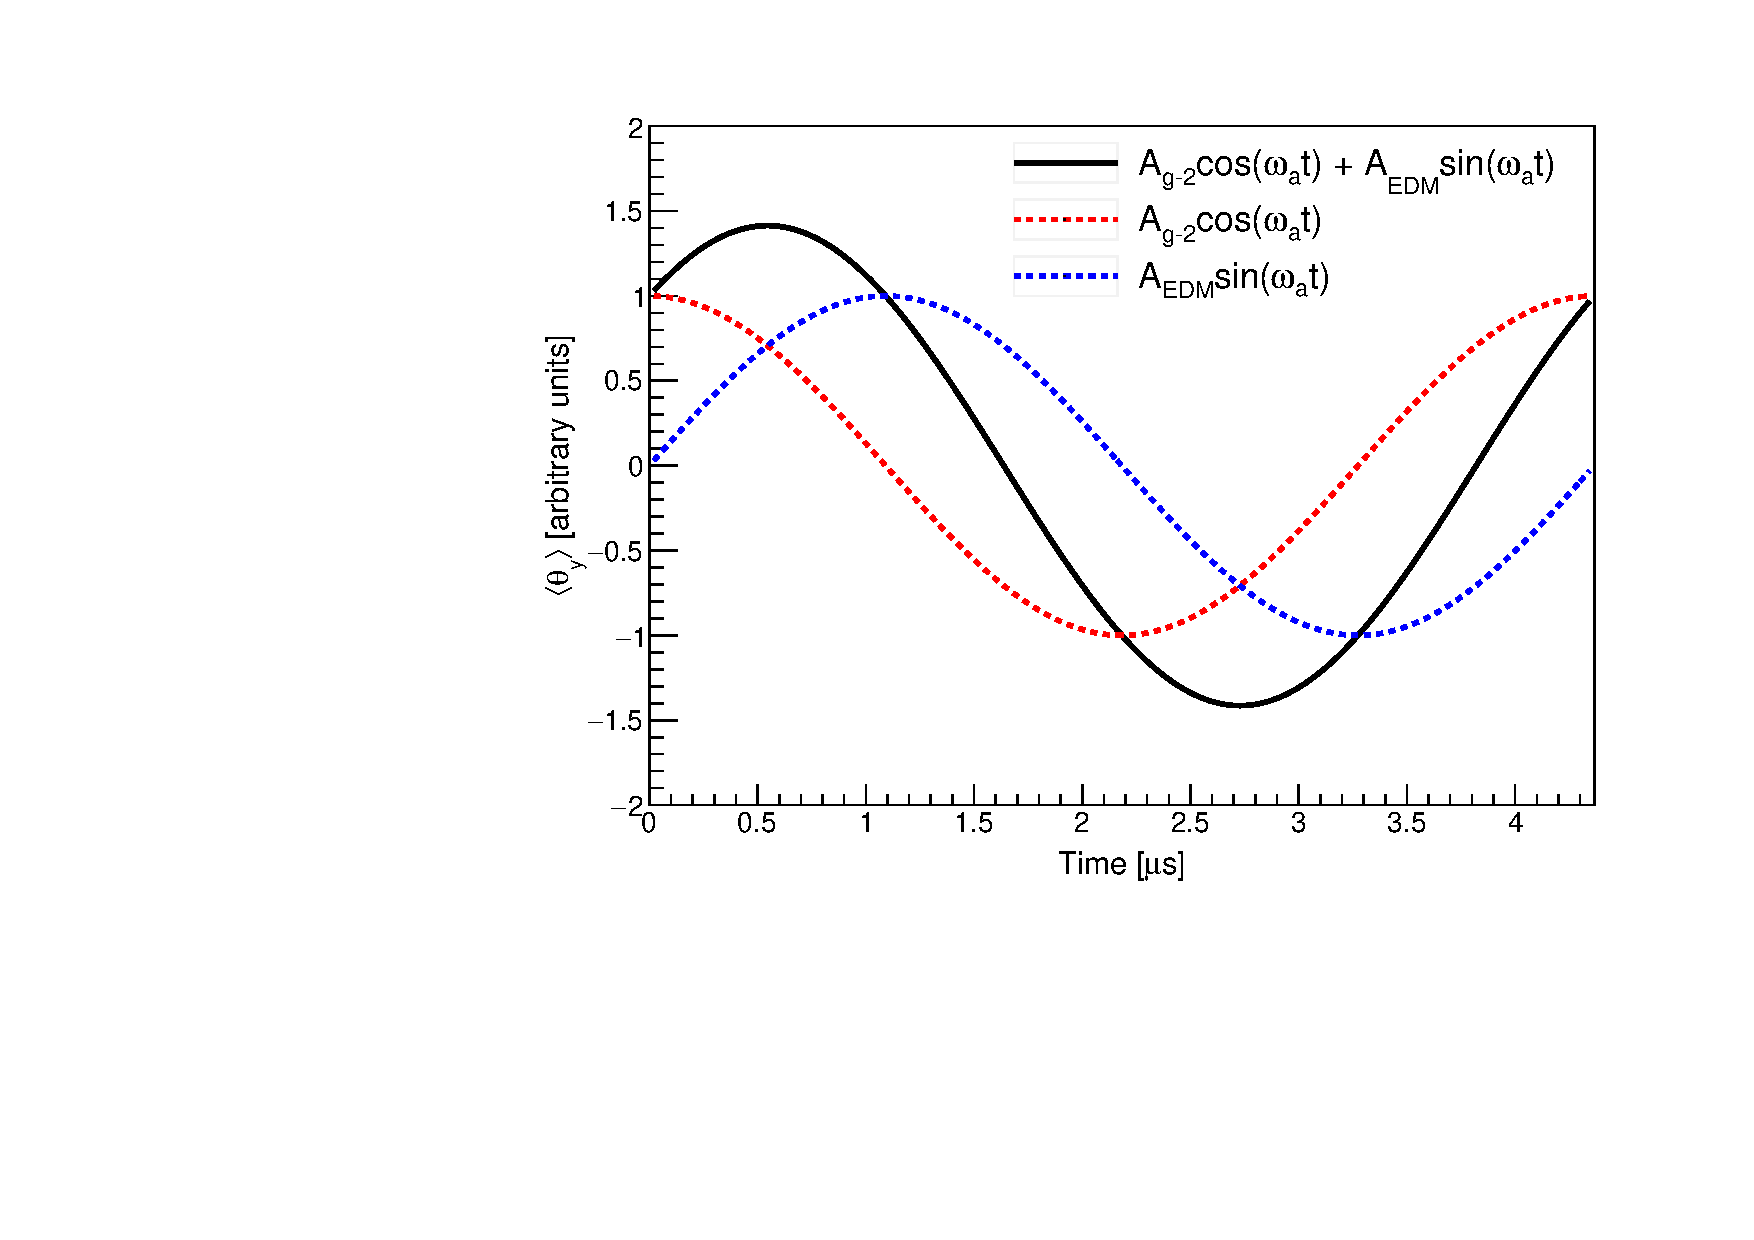
\includegraphics[trim={0 0 0 0},clip,width=0.69\textwidth]{Images/Chapter2/OrthogonalTermsIllustration.pdf}
\caption{An illustration of the average vertical angle fit function, Equation \ref{eqn:VertAngleFitFunc}, over a single $g-2$ period (\SI{4.365}{\micro\second}) compared with its individual orthogonal sine and cosine terms. The phase, $\phi$, and offset, $c$, are set to zero.}
\label{fig:OrthogonalTermsIllustration}
\end{figure}
%
where amplitudes $A_{g-2}$ and $A_{\text{EDM}}$ represent the observed angle in-phase with the $\omega_{a}$ ($g-2$) oscillation and the $\omega_{\eta}$ (EDM) oscillations respectively, and $\phi$ is the constant phase of the $\omega_{a}$ oscillation. It is assumed that $\omega_{a}>>\omega_{\eta}$, so the angular frequency of the oscillation is taken as $\omega_{a}$. The measured angle $A_{\text{EDM}}$ must then be corrected to obtain $\delta$, as will be expanded upon in the following section. The fit function, Equation \ref{eqn:VertAngleFitFunc}, is illustrated in Figure \ref{fig:OrthogonalTermsIllustration}.

\subsection{Sensitivity to a muon EDM}\label{subsec:EDMSensitivity}

The EDM search applies the same process of optimising the decay asymmetry and statistical sensitivity as the $\omega_{a}$ measurement, described in Section \ref{subsec:SensitivityToOmegaA}. The decay asymmetry function in this case relates to vertical (up/down) decays with a tilted spin precession plane, rather than the asymmetry for decays in the $x$-$z$ plane. A major point of difference here is that when the laboratory frame muon spin and momentum vectors are maximally aligned or anti-aligned, the boosted tilt angle is instantaneously zero. This means that there is no sensitivity to an EDM at maximum and minimum positron energy, which is reflected in the asymmetry function going to zero, as will be shown.

The time dependent probability of positron emission with a titled spin precession plane is given is given by
%
\begin{equation}
  P(\lambda^{*}, \theta^{*}, \phi^{*}, t) \propto N(\lambda^{*}) \Big( 1+A(\lambda^{*})\cos\alpha(\theta^{*}, \phi^{*}, t)\Big), 
\end{equation}
%
where $\theta^{*}$ and $\phi^{*}$ are the angles the positron momentum vector makes with the $z$ and $x$ axes in the rest frame, and $\alpha$ is the angle between the muon spin vector and the positron momentum vector, so that $\cos(\alpha)=\hat{s}\cdot\hat{p}$. The rest frame number and asymmetry functions, $N(\lambda^{*})$ and $A(\lambda^{*})$, are equal to those given in Equations \ref{eqn:N_restFrame} and \ref{eqn:A_restFrame}. Transforming into the laboratory frame, and integrating between $\lambda$ and 1, yields
%
\begin{equation}
  A(\lambda) = \frac{\sqrt{\lambda(1-\lambda)}(1-4\lambda)}{5+5\lambda-4\lambda^{2}},
  \label{eqn:AEDM_labFrame}
\end{equation}
%
with a statistical figure-of-merit (FOM) described by 
%
\begin{equation}
  NA^{2}(\lambda) \propto \frac{\lambda(1-\lambda)^{2}(1+4\lambda)^{2}}{5+5\lambda-4\lambda^{2}},
  \label{eqn:FOMEDM_labFrame}
\end{equation}
%
where $N(\lambda)$ is given by Equation \ref{eqn:N_labFrame}. A full derivation of the EDM asymmetry expressions by P. Debevec can be found in \cite{PaulEDMNote}. As illustrated in Figure \ref{fig:Asymmetry_EDM}, the FOM function indicates that statistical sensitivity to an EDM is highest at middling positron energy. The asymmetry and statistical FOM functions are verified in simulation in Chapter \ref{chap:5} Section \ref{sec:DecayAsymVerification}. 

\begin{figure}[t!]
\centering{}
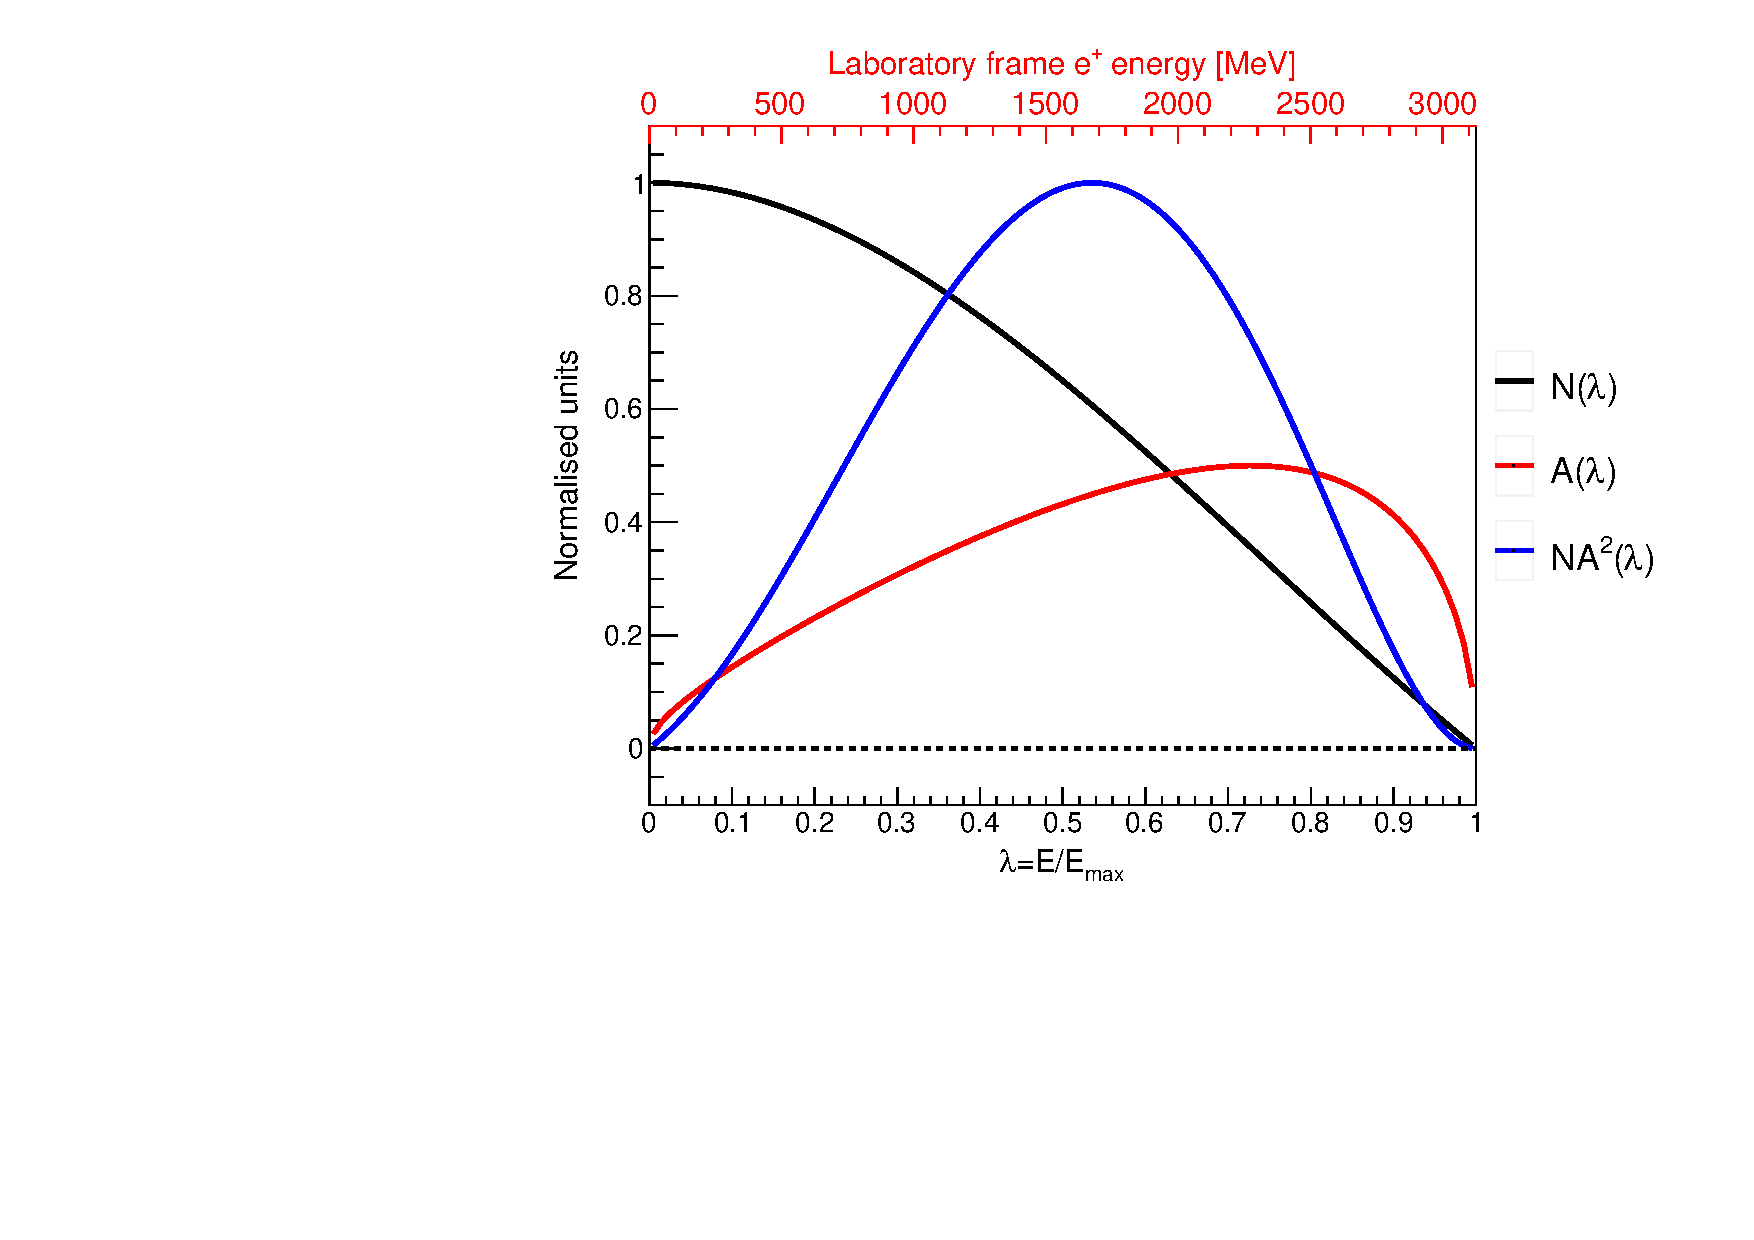
\includegraphics[trim={0 0 0 0},clip,width=.69\textwidth]{Images/Chapter2/Asymmetry_EDM_labFrame.pdf}
\caption{The number distribution function, $N(\lambda)$, the decay asymmetry function, $A(\lambda)$, and the statistical figure-of-merit function, $NA^{2}(\lambda)$, in the laboratory frame; for up/down decays and a non-zero muon EDM.}
\label{fig:Asymmetry_EDM}
\end{figure}

With a tilted precession plane, it might be expected that the size of average observed vertical angle in-phase with $\omega_{\eta}$, $A_{\text{EDM}}$ from Equation \ref{eqn:VertAngleFitFunc}, would follow the same dependence on energy as the asymmetry function described above. However, the Lorentz transformation into the laboratory frame results in a momentum dependent variation of the width of the vertical angle distribution, so that the average observed vertical angle is decreases with energy. A description of the variation of the maximum vertical angle with momentum, based on kinematic arguments, is given in Appendix \ref{app:MaxVertAngle}. In order to properly describe the variation of the angle associated with an EDM, both the asymmetry and the Lorentz transformation of the vertical angle must be accounted for. Following the derivation outlined by J. Price in \cite{JoeEDMNote}, the expression for the laboratory frame average vertical angle for decays occurring at the point of maximum tilt is given by 
%
\begin{equation}
  \langle {\theta_{y}^{\text{EDM}}} \rangle (\lambda) \propto \frac{(\lambda-1)(2\lambda+1)}{4\lambda^{2}-5\lambda-5} \frac{\sin{\delta^{*}}}{\gamma},
  \label{eqn:DilutionFunction1}
\end{equation} 
%
where $\sin{\delta^{*}}/\gamma \approx \delta$ by the small angle approximation. If all decays could be perfectly observed, and if $\delta^{*}$ were known, the above expression would describe the observed variation in the average vertical angle from an EDM exactly. The level of reduction of $\langle {\theta_{y}^{\text{EDM}}} \rangle $ compared to $\delta$ is termed `dilution', $d_{\text{EDM}}$, which may be expressed as a function of $\lambda$ by 
%
\begin{equation}
  d_{\text{EDM}}(\lambda) = \frac{1}{\delta} \cdot \langle {\theta_{y}^{\text{EDM}}} \rangle(\lambda),
  \label{eqn:DilutionFunction2}
\end{equation} 
%
and is generally referred to as the `dilution function' in this thesis. Efforts to characterise the dilution of $\delta$, with the inclusion of detector acceptance, is discussed in detail in Chapter \ref{chap:5}. An illustration of the dilution function, Equation \ref{eqn:DilutionFunction2}, is shown in Figure \ref{fig:DilutionFunc}.

\begin{figure}[t!]
\centering{}
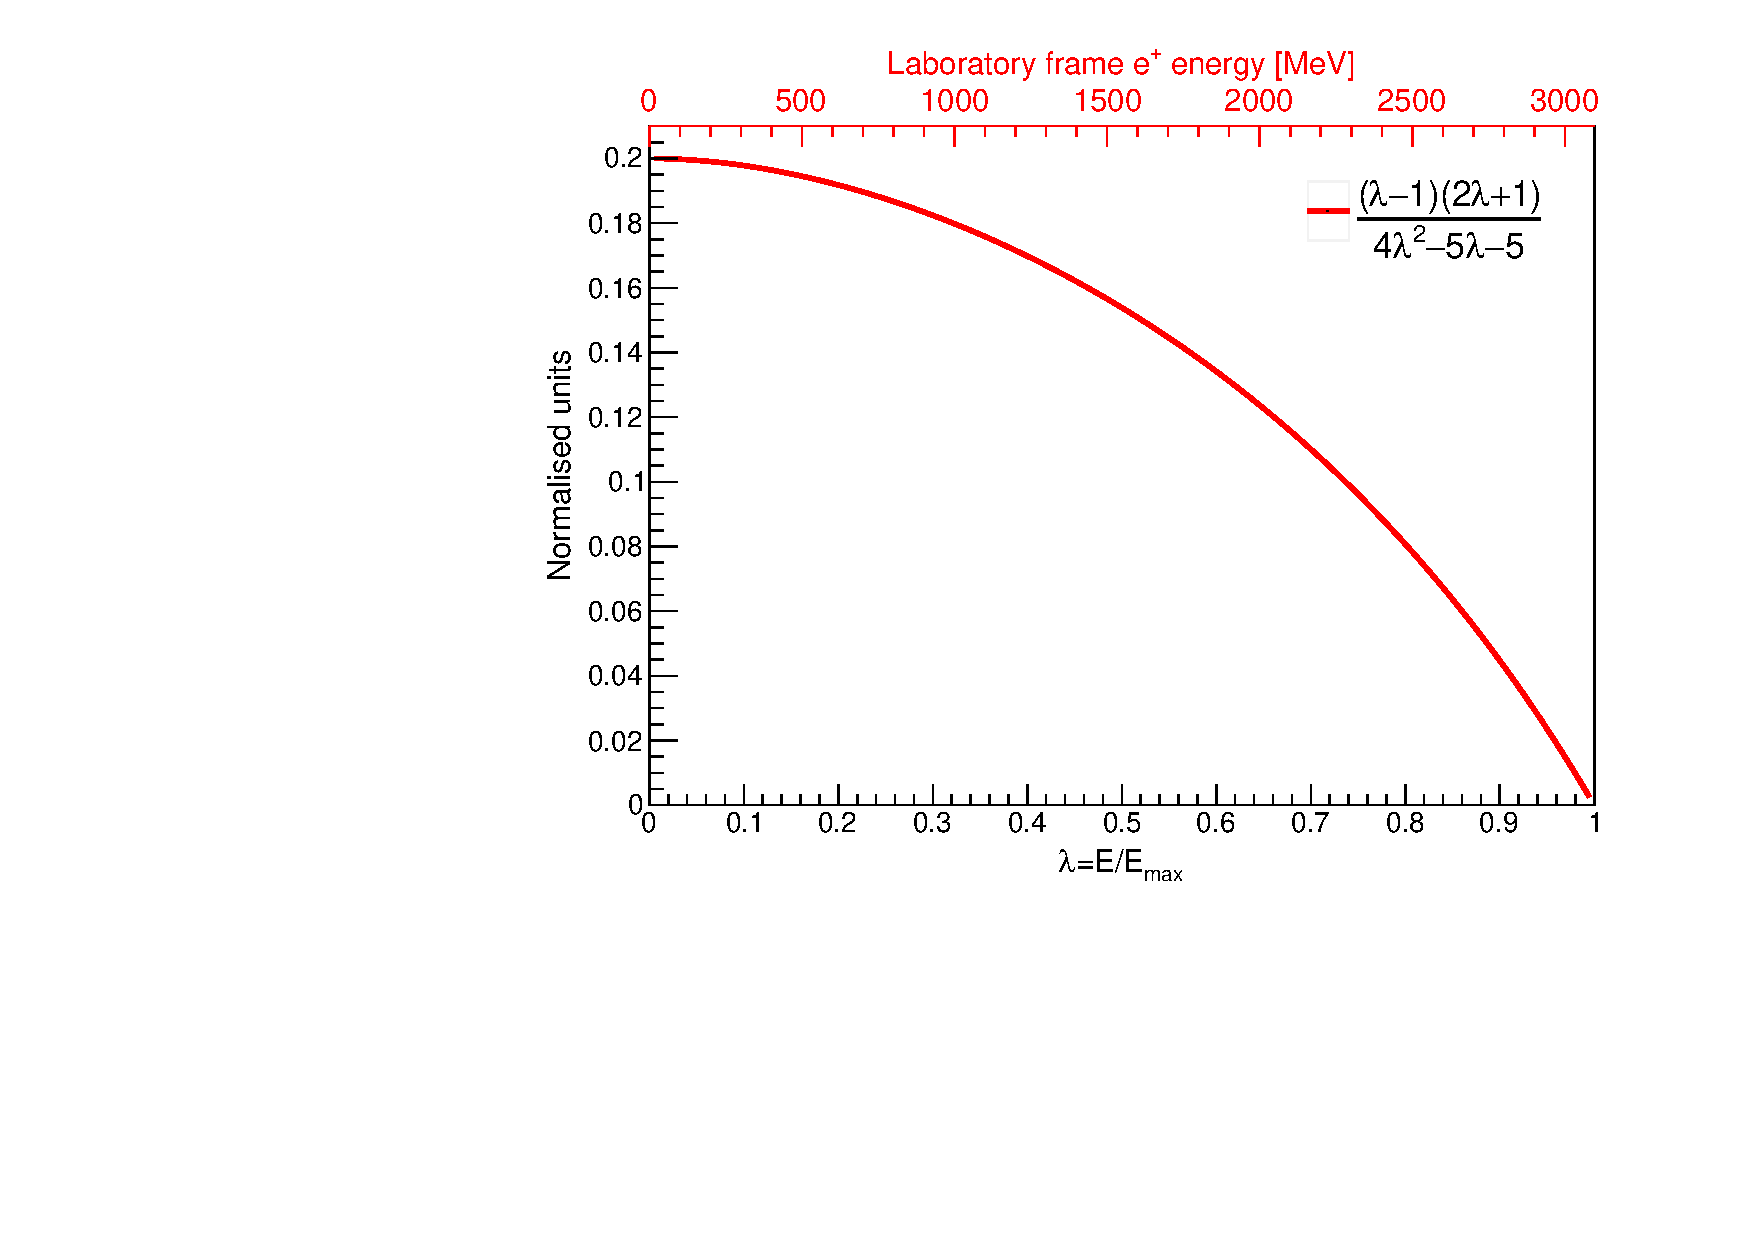
\includegraphics[trim={0 0 0 0},clip,width=0.65\textwidth]{Images/Chapter2/AverageAEDMFunction.pdf}
\caption{The normalised dilution function, Equation \ref{eqn:DilutionFunction2}, characterising the momentum dependant reduction in the observed angle, $A_{\text{EDM}}$, compared to laboratory frame tilt angle, $\delta$.}
\label{fig:DilutionFunc}
\end{figure}